% !TeX spellcheck = en_US
\documentclass[10pt,a4paper]{article}

\usepackage[utf8]{inputenc}
\usepackage[T1]{fontenc}	
\usepackage[italian]{babel}
\usepackage{amsmath}
\usepackage{amsfonts}
\usepackage{amssymb}
\usepackage{graphicx}

\usepackage[left=2cm,right=2cm,top=2cm,bottom=2cm]{geometry}
\geometry{a4paper}

\usepackage{booktabs} % for much better looking tables
\usepackage{verbatim}
\usepackage{subfig} % make it possible to include more than one captioned figure/table in a single 

\usepackage{fancyhdr} % This should be set AFTER setting up the page geometry
\pagestyle{fancy} % options: empty , plain , fancy
\renewcommand{\headrulewidth}{0pt} % customise the layout...
\lhead{}\chead{}\rhead{}
\lfoot{}\cfoot{\thepage}\rfoot{}

%%% SECTION TITLE APPEARANCE
\usepackage{sectsty}
%\allsectionsfont{\sffamily\mdseries\upshape} % (See the fntguide.pdf for font help)
% (This matches ConTeXt defaults)

% pacchetti che mi fanno schifo ma uso lo stesso (Bob è scemo...)
\renewcommand{\square}{ciao}
\usepackage[cdot, thickqspace, squaren]{SIunits}
% macro che mi piacciono
\def\code#1{\texttt{#1}}


\title{Esercitazione 5: Transistor JFET}

\author{Gruppo BE \\ Alessandro Candido, Roberto Ribatti}
\date{\today}
\begin{document}
\maketitle

\section{Scopo e strumentazione}
Studiare le caratteristiche e realizzare un amplificatore con il JFET a canale N 2N3819.
La strumentazione usata è quella presente sul banco di lavoro, più il suddetto transistor.

\section{Studio del funzionamento del JFET}

\subsection{Dimensionamento}
Si è montato il circuito in \figurename{\ref{fig:circuito1}}.

\begin{figure}[h!]
	\centering
	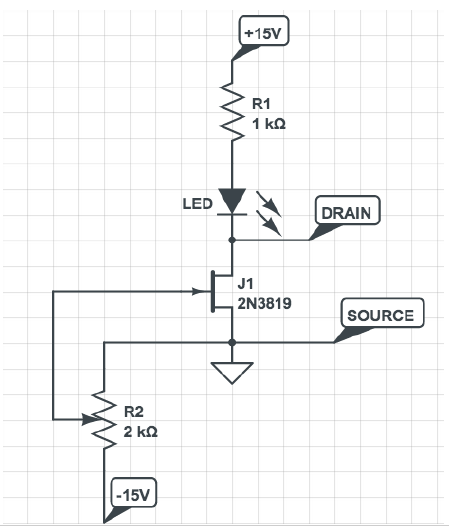
\includegraphics[width=0.5\textwidth]{../grafici/Circuito1.png}
	\caption{Circuito per lo studio del funzionamento del JFET}
	\label{fig:circuito1}
\end{figure}

I valori dei componenti usati sono stati misurati con il multimetro.

\begin{table}[h!]
	\centering
	\begin{tabular}{ccc}
		$V_{15} = \unit{15.0 \pm 0.2}{\volt}$  & $V_{-15} = \unit{-15.0 \pm 0.2}{\volt}$ & $R_1 = \unit{985 \pm 9}{\ohm}$
	\end{tabular}
\end{table}

\paragraph{LED} Il LED si accende e si spegne alla tensione $V_{GS} \sim \unit{1.89}{\volt}$. Infatti al di sopra di una certa tensione gate-source ($V_{GS}$) il canale è da considerarsi chiuso (pinch-off) e il transistor va in interdizione. Al di sotto della tensione di pinch-off a corrente inizia a scorrere nel canale, portando in conduzione anche il LED.

\subsection{Tensione di pinch-off $V_P$ e massima corrente di drain $I_{DSS}$}
I dati relativi alla curva $I_D - V_{GS}$ sono riportati in appendice in \tablename{\ref{njfet}}, il grafico relativo è invece riportato di seguito (\ref{fig:njfet}).

Si è trovato per la tensione di pinch-off il valore di $ $, mentre per la massima corrente di drain $ $.
% il valore sarà quello relativo alla corrente di 0.5uA; va notato che non c'è solo un errore sulla misura relativa alla tensione, ma c'è anche un errore dovuto a quanto è 0 la corrente di 0.5uA (entro l'errore lo è, ma magari con una misura più precisa quella corrente non sarebbe stata nulla e quindi anche la tensione sarebbe diversa, mantenendo il suo errore), andrebbe propagato anche quest'errore.
%stessa cosa per idss
%queste considerazioni espresse meglio andrebbero poi scritte nella relazione

%includere il grafico

\section{Montaggio amplificatore}


\section{Misure a frequenza fissa}

\section{Impedenza d'ingresso}

\section{Aumento del guadagno}

\pagebreak
\section{Appendice: Dati}
Si riportano qui le tabelle di dati usati per i fit e i grafici.

\begin{figure}[h]
	\centering
	\begin{minipage}[c]{0.4\textwidth}
		\centering
		%\input{../tabelle/tab_guadagnopiccolisegnali_ol.txt}
		\captionof{table}{Curva $I_D - V_{GS}$}
		\label{njfet}
	\end{minipage}
	\begin{minipage}[c]{0.4\textwidth}
		\centering
		%\input{../tabelle/tab_f_domain.txt}
		\captionof{table}{}
		\label{}
	\end{minipage}
\end{figure}

\end{document}
